\chapter{Discriminant analysis}
\label{discriminant}

Discriminant analysis presupposes that we have a number of known groups of individuals, and a set of data which has been collected on individuals within these groups.   We wish to find a way of using that data to predict which group these individuals belong to, either to understand the differences or to be able to predict group membership.  \cite{Bumpus:1898} collected data on sparrows who survived and didn't survive a storm, these data are extensively analysed in this context by Manly, the primary aim of the analysis being to look for differences between the groups.   Are there different features which help us tell storm survivors from non-survivors?   More usually, we may be interested in predicting group membership.   Common examples can be found in finance; can banks tell good credit risks from bad based on data collected on customers who have subsequently defaulted on loans, see \cite{Johnson+Wichern:2002} for more details.   Another good account of discriminant analysis is given by \cite{Flury:1997} who suuggests it may be valuable when we have to carry out destructive procedures to determine group membership (such as in certain quality control investigations).  Finally a rather brief account is given in \cite{Venables+Ripley:2002}, which gives the example of disease diagnosis.   Consider a set of measurements of patient characterstics, and information determined on whether these patients have breast cancer or not.   We would be very interested in being able to make a determination of breast cancer based on the data, rather than having to wait for biopsy or other pathological information.

Discriminant analysis in one dimension seems straightforward enough.   We can examine the densities of the two groups and find an optimal cut-off point, which classifies the two groups as accurately as possible.   Some idea of the procedure is given in figure \ref{discrim}, which illustrates the idea behind discriminant function.

\begin{figure}
\begin{center}
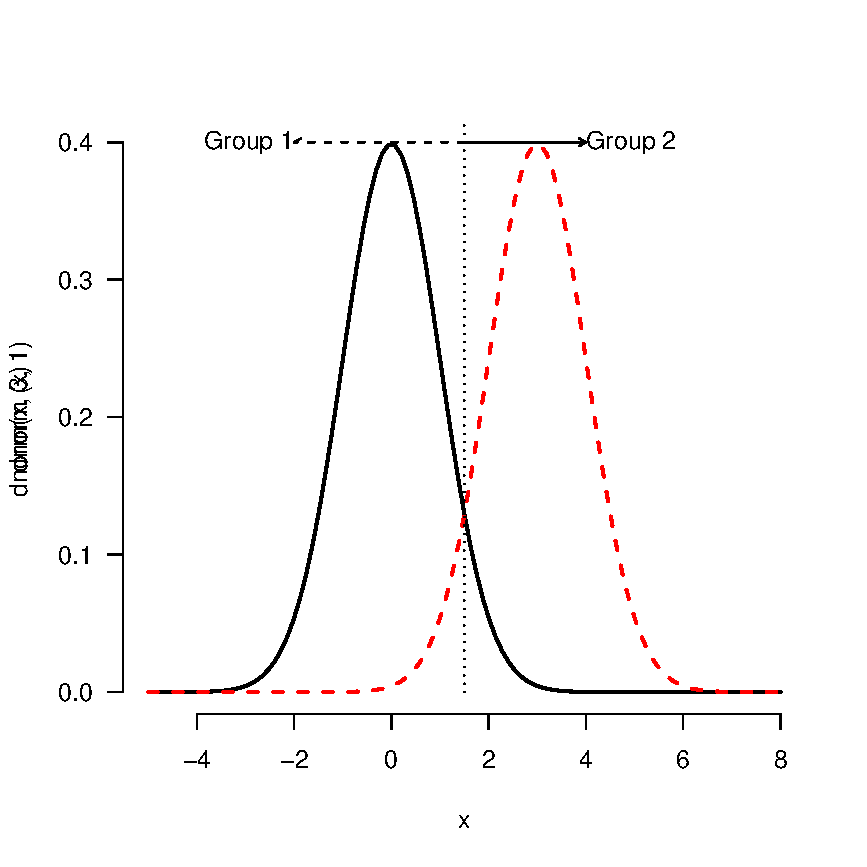
\includegraphics[width = 0.5\textwidth]{images/discrim}
\caption{Idealised discrimant function}
\label{discrim}
\end{center}
\end{figure}

Note immediately that there is a measureable risk of misclassification, which depends on the variance within groups and the separation between groups.   All we need to do is extent this procedure to work in more than one dimension.   We are going to realise this by seeking a linear combination giving us the largest separation between groups.   In other words, we are going to find linear combinations based on the original variables:

\begin{equation}
z = a_{1} x_{1} + a_{2} x_{2} + \ldots + a_{p} x_{p}
\end{equation}


However our linear combination this time will be optimised to give us the greatest potential for distinguishing the two groups.   Having found a suitable linear combination, we select a cut-off point (denoted by the vertical dotted line in the figure above), and assign observations to group 1 or group 2 based on the value relative to the cut-off.   You can see from the stylised function shown that some observations will be misclassfied!   We check the performance of this aspect of our procedure by means of a confusion matrix.


Recall that when conducting the $T^{2}$ test we essentially looked for linear combination of variables which maximised the difference between groups.   Similar ideas apply in discriminant analysis.   We seek a transformation of the data which gives the maximum ratio of group means to group variance within the two groups, i.e. we are maximising the between group variation relative to the within group variance - this should sound vaguely like what goes on in ANOVA:


\begin{tabular}{llll}
Source & d.f. & Mean Square & F ratio \\
\hline
Between groups & $m-1$ & $M_{B}$ $M_{B} / M_{W}$\\
Within groups & $N-m$ & $M_{W}$ & \\
 & N-1 & & \\
\end{tabular}

We need to find a linear combination that yields as large an F ratio as possible, hence the coefficients $a_{1}, \ldots, a_{p}$ need to be chosen to maximise this value.   More than one discriminant function is available, there are

\begin{equation}
s = min(p, m-1)
\end{equation}
discriminant functions available, where $p$ is the number of variables, and $m$ is the number of groups.

Considering the case where we have $m > 2$ groups, and $p > 2$ variables, we are looking for the following discriminant functions:


\begin{eqnarray*}
z_{1} &=& a_{11}x_{1} + a_{12}x_{2} + \ldots + a_{1p}x_{p}\\
z_{2} &=& a_{21}x_{1} + a_{22}x_{2} + \ldots + a_{2p}x_{p}\\
\ldots\\
z_{s} &=& a_{s1}x_{1} + a_{s2}x_{2} + \ldots + a_{sp}x_{p}
\end{eqnarray*}

although hopefully only  a small number of these linear combinations will account for all important differences between groups.

\section{Fisher discimination}
%\section{Fisher, linear and quadratic discimination}
\label{fisherdisc}

Remember the $T^{2}$ statistic:

\begin{equation}
T^{2}(\boldsymbol{a}) = \frac{ \left( \boldsymbol{a} (\boldsymbol{\bar{x}}_{1} - \boldsymbol{\bar{x}}_{2} ) \right)^{2} n_{1}n_{2}/(n_{1}+n_{2})}{\boldsymbol{a}^{T}\boldsymbol{S}\boldsymbol{a}}
\end{equation}

This is equivalent to finding $\boldsymbol{a}$ which maximises $|\boldsymbol{a} (\boldsymbol{\bar{x}}_{1} - \boldsymbol{\bar{x}}_{2} ) |$ subject to $\boldsymbol{a}^{T}\boldsymbol{S}\boldsymbol{a}$ = 1.   This has a single solution:

\begin{displaymath}
\boldsymbol{a} = \boldsymbol{S}^{-1}(\boldsymbol{\bar{x}}_{1} - \boldsymbol{\bar{x}}_{2} )
\end{displaymath}

and so the linear discriminant function is given by:

\begin{displaymath}
z = (\boldsymbol{\bar{x}}_{1} - \boldsymbol{\bar{x}}_{2} )^{T}\boldsymbol{S}^{-1} \boldsymbol{x}
\end{displaymath}

In two dimensions, an obvious cut-off would be the midpoint between the mean value of $z$ for group 1 and 2.


Fisher's approach has been extended to cope with more than two groups.  Again, we wish to find a linear combination $z = \boldsymbol{a}^{T} \boldsymbol{x}$ which maximised the ratio of between group variance to within group variance.

If we calculate the within sample matrix of sum of squares and cross products $\boldsymbol{W}$, and the total sample matrix of sum of squares and cross products $\boldsymbol{T}$, we can easily find the between-groups sample matrix sum of squares and cross products:

\begin{equation}
\boldsymbol{B} = \boldsymbol{T} - \boldsymbol{W}
\end{equation}



In effect we wish to maximise:

\begin{equation}
\frac{ \boldsymbol{a}^{T} \boldsymbol{B} \boldsymbol{a}}{ \boldsymbol{a}^{T} \boldsymbol{W} \boldsymbol{a}} 
\end{equation}
and usually do this subject to the condition that $\boldsymbol{a}^{T} \boldsymbol{W} \boldsymbol{a}$ = 1.   Fisher's method of discriminant analysis reduces to finding the eigenvalues and corresponding eigenvectors of $\boldsymbol{W}^{-1}\boldsymbol{B}$.   The ordered eigenvalues $\lambda_{1}, \ldots, \lambda_{s}$ are the ratio of between groups to within groups sum of squares and cross products for $z_{1}, \ldots, z_{s}$, the corresponding eigenvectors, $\boldsymbol{a}_{1}, \ldots, \boldsymbol{a}_{s}$, where $\boldsymbol{a}_{i} = \left( \begin{array}{c} a_{i1} \\ \vdots \\ a_{ip} \end{array} \right)$ are the coefficients of $z_{i}$.

We make a number of big assumptions in discriminant analysis: that observations are a random sample, that they are normally distributed and that the variance is the same for each group.   Discriminant analysis is relatively resistant to some departures from the normality assumption - it can cope with skewness but not with outliers.   %Some transformation of the data may be necessary in this situation.   It is also possible to use prior information to deal with unequal sample sizes.



%\begin{displaymath}
%W = \frac{ (\boldsymbol{X} - \boldsymbol{C} \boldsymbol{\bar{X}_{Class}})^{T} (\boldsymbol{X} - \boldsymbol{C} \boldsymbol{\bar{X}_{Class}})}{n-c}
%\end{displaymath} 

%\begin{displaymath}
%B  = \frac{  (\boldsymbol{C \bar{X}_{Class}} - \boldsymbol{I \bar{X}})^{T}(\boldsymbol{C \bar{X}_{Class}} - \boldsymbol{I \bar{X}})}{c-1}
%\end{displaymath} 

%where $\boldsymbol{\bar{X}_{Class}}$ are the mean values in a group denoted by $\boldsymbol{C}$, and $\boldsymbol{\bar{X}}$ are the overall means for data matrix $\boldsymbol{X}$.   $n$ denotes the number of individuals observed, $c$ the number of classes.



%\begin{displaymath}
%z = \alpha_{1} x_{1} + \alpha_{2} x_{2} + \ldots + \alpha_{p} x_{p}
%\end{displaymath}




%In principle, we need to carry out an eigen decomposition of the matrix $\boldsymbol{W^{-1}B}$ (although in modern computational practice a lot of the details are different, for example some rescaling goes on so that the within-group covariance is set to be $\boldsymbol{I}$).   The linear combination obtained are referred to by Manly as the canonical discriminant functions.   These linear combinations have within group variance $\boldsymbol{a^{T} W a}$ and between group variance  $\boldsymbol{a}^{T} \boldsymbol{B a}$, with the total variance given by:

%\begin{displaymath}
%\boldsymbol{a}^{T} \boldsymbol{S a}  = \frac{(n - g) \boldsymbol{W} + (g - 1) \boldsymbol{B}}{n - 1}
%\end{displaymath}





\section{Accuracy of discrimination}  
\label{accuracy}

Clearly, one important measure of the success of our discriminant rule is the accuracy of group prediction: note that there are a number of ways of measuring this and that discriminant analysis is one technique among many used in \emph{supervised classification}.   There are many techniques in machine learning and other areas which are used for classification, for example you have already met the technique of logistic discrimination.   

Model over-fitting is a known problem: we can fit a classifier really really well to our existing data but it doesn't work well next time we carry out a data collection exercise.   A key concept in this regard is the use of training and testing sets, where we split our data into two groups, and use one part to build a classifier, and the other to test it.   There are many other technques which can help in this regard, for example leave one out (loo) cross validation and some of the more recent multivariate texts should be consulted.

An important idea in terms of measuring the success of our classifier is the \emph{confusion matrix}.   This sounds rather grand, but is basically a matrix telling us how many times our discriminant function made a correct classification, and how many times it got it wrong.

\section{Importance of variables in discrimination}
\label{imporvar}

Some textbooks refer to questions surrounding selection of variables for use in a classifier.   It is important to consider whether variables are necessary for classification; often a tolerance test may be used prior to the analysis to remove multicollinear and singular variables.   It may even be desirable to carry out a dimension reducing technique.   The reason for carrying out these tests are related to over-fitting.

Some software provides ``standardised'' coefficients, the idea being that perhaps it is safe to remove variables with small standardised coefficients.   However, another approach could well be to consider classifiers with different numbers and combinations of variables and contrast the confusion matrix.   This might help identify variables which do the best job of distinguishing the groups, and those which are the least necessary.

%If $D^{2}$ is large if the discriminant function performs well.   
%Wilks' $\Lambda$ is used to assess the importance of variables: the smaller it is the more important the variable is (there are associated F statistics and p values to help in this regard).

\section{Canonical discriminant functions}
\label{candisc}

As mentioned earlier, we can have more than one discriminant function.   It is usual to plot these on a scatterplot in an attempt to visualise the discriminant ability.   However, there are tests of significance.

For example, we wish to find discriminants with a small Wilk's lambda ($\frac{|\boldsymbol{W}|}{|\boldsymbol{T}|}$), in our case this can be derived as :

\begin{equation}
\Lambda^{2} = \left( \sum_{k=1}^{m} n_{k} - 1 - \frac{1}{2}(p + m) \right) \ln (1 + \lambda_{j}),
\end{equation}
which has a $\chi^{2}$ distribution with $p + m - 2j$ degrees of freedom.


%\section{Logistic discrimination}
%\label{logdisc}

%\section{Dimension reduction and discriminant analysis}
%\label{drdisc}







\section{Linear discrimination - a worked example}

In practice, we're going to consider a classification exercise on the Iris data.   This is rather well known data featuring three species of Iris, and four anatomical measures.   First of all we need to load the \texttt{MASS} to obtain the \texttt{lda()} function.   Then we are going to pull out a training set from the Iris data.

\singlespacing
\begin{verbatim}
> library(MASS)
>  data(iris3)
>  Iris <- data.frame(rbind(iris3[,,1], iris3[,,2], iris3[,,3]),
+                         Sp = rep(c("s","c","v"), rep(50,3)))
>      train <- sample(1:150, 75)
\end{verbatim}
\onehalfspacing

\texttt{train} is a set of index numbers which will allow us to extract a training set.   We use \texttt{lda()} to fit a discriminant analysis, setting all priors equal to 1 (i.e. group memberships the same), and \texttt{subset = train} to fit the analysis to the training set.   The squiggle dot indicates that we wish to use all other variables within Iris to predict Species (Sp).

\begin{verbatim}
> z <- lda(Sp ~ ., Iris, prior = c(1,1,1)/3, subset = train)
> z
\end{verbatim}


Having extracted a training set, we are going to classify the remaining Iris' and see how well the predicted and actual species line up.

\singlespacing
\begin{verbatim}
> actual <-  Iris[-train,]$Sp
> preds <- predict(z, Iris[-train, ])$class)
> xtabs(~actual + preds)
\end{verbatim}
\onehalfspacing


One little thing to watch when using software is that in practice, Fisher's approach tends not to be used.   An approach based on probability distributions and using Bayes rule is common.   All this does, is correct for the proportions in each group to start with.   Instead of finding a discriminant rule assuming a 50:50 split, we use information on more plausible group numbers.

%%% Local Variables: ***
%%% mode:latex ***
%%% TeX-master: "../book.tex"  ***
%%% End: *** 